\chapter{Description du code Numérique}\label{sec:nbody-readme}
Le but de cette partie est de présenter les différentes options du code modifié. Ces options sont lues à partir d'un fichier commun \textbf{disk.in}. Si une option n'est pas présente, la valeur par défaut sera lue à partir du code. Le fichier \textbf{disk.out} récapitule toutes les valeurs de toutes les options et paramètres effectifs du code. Des paramètres du fichier \textbf{disk.in} peuvent donc ne pas être présent car l'option est inactive, et des valeurs par défaut qui n'étaient pas présentes dans \textbf{disk.in} peuvent apparaître dans le fichier de sortie.

Il est possible de mettre des commentaires dans le fichier \textbf{disk.in}, que ce soit pour commenter une ligne entière, ou pour mettre en fin de ligne après un paramètre, à l'aide du caractère \og !\fg exactement comme en \textbf{Fortran 90}.

Le code est en grande partie le code Mercury \cite{chambers1999hybrid}. Les effets du disque ont été inclus dans la partie \textbf{mfo\_user} prévue pour inclure des effets propre à chaque utilisateur. 

Pour autant, le code a été conçu de manière modulaire en portant une attention particulière au temps d'exécution et à la
souplesse d'utilisation. La plupart des effets sont désactivables par une simple option dans un fichier de paramètres spécifique
aux effets du disque \textbf{disk.in}. 

Prenons un exemple. Le couple exercé par le disque sur la planète peut être issu des formules de \cite{paardekooper2011torque}, ou bien suivre plusieurs lois artificielles permettant de tester certains effets dans des cas simplifiés. Pour autant, cette souplesse d'utilisation ne se fait pas au détriment de la célérité du code, car au lancement de ce dernier, les options sont lues et des pointeurs de fonctions permettent au code d'exécuter directement la bonne fonction lors de l'intégration, sans avoir à tester à chaque pas de temps quelle fonction doit être lancée. 

\section{Paramètres divers}
Ici, je regroupe des paramètres du disque qui nécessitent simplement une valeur : 
\begin{verbatim}
b/h = 0.6
adiabatic_index = 1.4
mean_molecular_weight = 2.35
disk_edges = 0.1 100.
sample = 800
\end{verbatim}

\textbf{b/h} est le paramètre de lissage du potentiel gravitationnel d'une planète (qui diverge dans les simulations hydrodynamiques et qui est un paramètre des formules de \cite{paardekooper2011torque}.

\textbf{adiabatic\_index} est l'indice adiabatique $\gamma$ comme son nom l'indique. De même, \textbf{mean\_molecular\_weight} est la masse moléculaire moyenne $\mu$.

\textbf{disk\_edges} définit les deux extrémités du disque, les bords interne et externe.

\textbf{sample} définit le nombre de points qu'auront les profils radiaux des différents paramètres du disque. Ces points ne sont pas répartis uniformément, il y a plus de points au bord interne qu'au bord externe, afin d'avoir une évolution plus fine des paramètres en fonction du rayon.

\section{Densité de surface}
\textbf{surface\_density} permet de définir le profil en loi de puissance pour la densité de surface : 
\begin{verbatim}
surface_density = 500 0.5
\end{verbatim}
Ici, on a défini le profil suivant : 
\begin{align*}
\Sigma(R) &= 500. \cdot R^{-0.5} \unit{g/cm^2}
\end{align*}

Mais il est aussi possible de donner un profil tabulé de densité de surface en fonction du rayon en paramètre d'entrée, en spécifiant le paramètre suivant : 
\begin{verbatim}
surface_density = manual
\end{verbatim}
Ainsi, le profil de densité de surface sera lu à partir du fichier \textbf{surface\_density\_profile.dat} qui doit être constitué de deux colonnes, la première étant la valeur du rayon en \unit{UA}, et la deuxième la densité de surface en \unit{g/cm^2}. Les lignes doivent être classées par ordre croissant de distance orbitale. (les premières lignes étant les points les plus proches de l'étoile, et les dernières les points les plus lointains. 

\begin{remarque}
Une interpolation sera réalisée si la discrétisation du fichier d'entrée est différente de celle du code.
\end{remarque}

\bigskip

À ceci s'ajoute un paramètre supplémentaire : 
\begin{verbatim}
inner_smoothing_width = 0.05
\end{verbatim}

Ce paramètre représente la longueur d'amortissement de la densité de surface au bord interne du disque, afin que la densité de surface au bord interne soit très faible. Cette longueur est exprimée en pourcentage de distance orbitale du bord interne ; c'est-à-dire que si le bord interne est à $0.1\unit{UA}$, alors dans le cas présent, le lissage sera effectué sur une longueur de $0.005\unit{UA}$.

\section{Irradiation de l'étoile centrale}\index{irradiation}
\textbf{is\_irradiation} permet de définir si on veut inclure ou non l'irradiation dans le calcul de l'équilibre énergétique du disque. 

\begin{verbatim}
is_irradiation = 1
disk_albedo = 0.5
r_star = 4.65e-3 ! AU
t_star = 5700 ! K
\end{verbatim}

Les paramètres sont relativement explicites mais pour détailler, \textbf{disk\_albedo} est l'albédo moyen du disque protoplanétaire, il représente le fait qu'une partie de la lumière incidente de l'étoile est directement réfléchie vers l'espace.

\textbf{r\_star} et \textbf{t\_star} sont respectivement le rayon de l'étoile en \unit{UA} et sa température en Kelvin.

La manière dont est modélisée l'irradiation de l'étoile centrale est détaillée dans \refsec{sec:irradiation}.

\section{Viscosité}
Il est possible de définir plusieurs types de viscosité via l'option \textbf{viscosity\_type} : \textbf{constant}, \textbf{alpha} et \textbf{alpha\_dz}.

\subsection{constant}
Ce paramètre permet de définir une viscosité $\nu$ constante dans tout le disque. La valeur de la viscosité associée est définie dans le paramètre \textbf{viscosity} en \unit{cm^2/s}.

\begin{verbatim}
viscosity_type = constant
viscosity = 1e15 ! cm^2/s
\end{verbatim}

\subsection{alpha}
Ce paramètre permet de définir une viscosité via la prescription alpha de \cite{shakura1973black}. La valeur du paramètre alpha sera lue dans le paramètre \textbf{alpha}. 

\begin{verbatim}
viscosity_type = alpha
alpha = 5e-3
\end{verbatim}

\subsection{alpha\_dz}\label{sec:dead_zone}\index{zone morte}
Ce paramètre permet de définir une viscosité alpha par morceau, permettant de modéliser une zone morte. On aura donc 3 zones
avec 3 valeurs d'alpha différentes. Pour définir ces zones-là, il faut donner dans le paramètre \textbf{alpha\_dz} trois valeurs
de $\alpha$ et dans \textbf{radius\_dz} deux valeurs de distance orbitale (en \unit{UA}) pour définir les bornes de la zone
morte.
\begin{verbatim}
viscosity_type = alpha_dz
alpha_dz = 0.005 0.0001 0.005
radius_dz = 1.0 10.0 ! in AU
\end{verbatim}

Quand cette option est activée, une modification au profil de densité est appliquée, afin de modéliser une sous-densité, puis une sur-densité avant et après le bord interne de la zone morte. L'écart maximum de ces bosses est de 15\% de la valeur de la densité au bord interne de la zone morte. 

À ceci s'ajoute un lissage des valeurs de $\alpha$ entre la valeur à gauche et la valeur à droite de la transition selon une tangente hyperbolique. La transition s'effectue typiquement sur une longueur égale à 10\% de la position de la transition dans le disque (si la transition est à $1\unit{UA}$, alors la transition a lieu sur $0.1\unit{UA}$ autour de la transition).

\section{Opacité}\index{opacité}
Afin de pouvoir les comparer, j'ai ajouté au code la possibilité de tourner avec différents modèles pour l'opacité. 

Les différents modèles sont \citep{bell1994FU, zhu2009nonsteady, chambers2009analytic, hure2000transition}

\subsection{bell}
\begin{verbatim}
opacity_type = bell
\end{verbatim}

L'opacité est alors calculée en utilisant le modèle fourni par \cite{bell1994FU}. 

\subsection{zhu}
\begin{verbatim}
opacity_type = zhu
\end{verbatim}

L'opacité est alors calculée en utilisant le modèle fourni par \cite{zhu2009nonsteady}. 

\subsection{chambers}
\begin{verbatim}
opacity_type = chambers
\end{verbatim}

L'opacité est alors calculée en utilisant le modèle fourni par \cite{chambers2009analytic}. Ce modèle est très simplifié et
utilise une opacité constante sur un grand régime de température, pour ensuite faire une transition vers une loi de puissance à
très haute température.

\subsection{hure}
\begin{verbatim}
opacity_type = hure
\end{verbatim}

L'opacité est alors calculée en utilisant le modèle fourni par \cite{hure2000transition}. 

À la différence de tous les autres modèles que j'ai implémenté, celui de \cite{hure2000transition} est directement une table d'opacité, sans faire intervenir de loi de puissance pour différents régimes. Il n'introduit donc pas d'incertitudes supplémentaires via les lois de puissance qu'il définit. Cette table
d'opacité de Rosseland correspond à la composition suivante $X=0.70$, $Y=0.28$ et $Z=0.02$ et est basée sur
\cite{seaton1994opacities, alexander1994low, henning1996dust}.

En effet, dans le cas qui nous intéresse, c'est-à-dire la migration planétaire via la formule de \citep{paardekooper2011torque},
l'indice des lois de puissance pour la densité de surface et la température a une très grande influence sur la couple effectif
du disque. Et les transitions d'opacité, très marquées lors de la transition des lois de puissance, font apparaître des zones
particulières dans le disque qui n'ont parfois aucune réalité physique, mais ont de grandes conséquences sur le résultat des
simulations. De même, le lissage qu'elles introduisent masque certaines zones d'intérêt qui ne sont mises en évidence qu'avec
une table d'opacité où tous les effets fins ont été préservés.

\section{Turbulence}
Pour activer la turbulence dans le disque, c'est-à-dire l'effet que la turbulence peut induire sur la migration planétaire, il suffit d'utiliser le paramètre suivant : 
\begin{verbatim}
is_turbulence = 1
\end{verbatim}

La turbulence n'est ici qu'une migration stochastique de moyenne nulle qui perturbe les planètes et leur migration. 

Le modèle utilisé est le même que celui détaillé dans \cite{ogihara2007accretion}. Le principe est de définir un potentiel
turbulent dans le disque, fait de la superposition de perturbations individuelles qui ont des modes $m$, temps de vie $t_m$ et
position dans le disque différents. 

Dans le cas typique, il y a 100 modes différents dans le disque : 
\begin{align}
\Phi_\text{turb}(R,\phi,t) &= \gamma R^2 \Omega^2 \sum_{k=1}^{100} \Lambda_k(R,\phi,t)
\end{align}
avec 
\begin{align}
\Lambda_k &= \xi_k e^{-\frac{(R-R_k)^2}{{\sigma_k}^2}} \cos\left(m_k \phi -\phi_k - \Omega_k\tilde{t}_k\right) \sin\left(\pi \tilde{t}_k/\Delta t_k\right)
\end{align}

$\xi_k$ est une constante adimensionnée déterminée aléatoirement en suivant une distribution gaussienne.

$R_k$ et $\phi_k$ sont respectivement les coordonnées radiales et azimutales du mode $k$ choisies aléatoirement et de manière uniforme pour l'un entre les bornes du disque, pour l'autre entre $0$ et $2\pi$. 

Chaque mode $k$ possède un nombre de modes $m_k$ déterminé aléatoirement selon une distribution logarithmique entre $m=1$ et
$m=150$. Ce nombre de modes $m_k$ détermine l'extension radiale et la durée du vie du mode $k$.

$\sigma_k = \pi R_k / 4m_k$ est l'extension radiale de ce mode tandis que $\Omega_k$ représente la vitesse angulaire képlerienne à la position $R=R_k$.

$\Delta t_k=0.2\pi R_k / m_k c_s$ est la durée de vie du mode $k$. 

\bigskip

Les modes apparaissent et disparaissent en fonction de leur temps de vie et sont remplacés afin qu'il y ait toujours 100 modes différents dans le disque à un instant $t$. Chaque mode $k$ est créé à un instant $t_{0,k}$ et se termine quand $\tilde{t}_k = t-t_{0,k} > \Delta t_k$, l'extension du mode et son temps de vie ne dépendent pas du nombre total $k$ de modes.

\section{Migration}\index{migration!Type I}
\subsection{real}
C'est le cas le plus classique. Il n'y a pas besoin de définir d'autres paramètres, la migration induite par le disque de gaz sera simplement calculée à partir du modèle de \cite{paardekooper2011torque}.

\begin{verbatim}
torque_type = real
\end{verbatim}

\subsection{mass\_dependant}\label{sec:mass_dependant}
\begin{figure}[htbp]
\centering
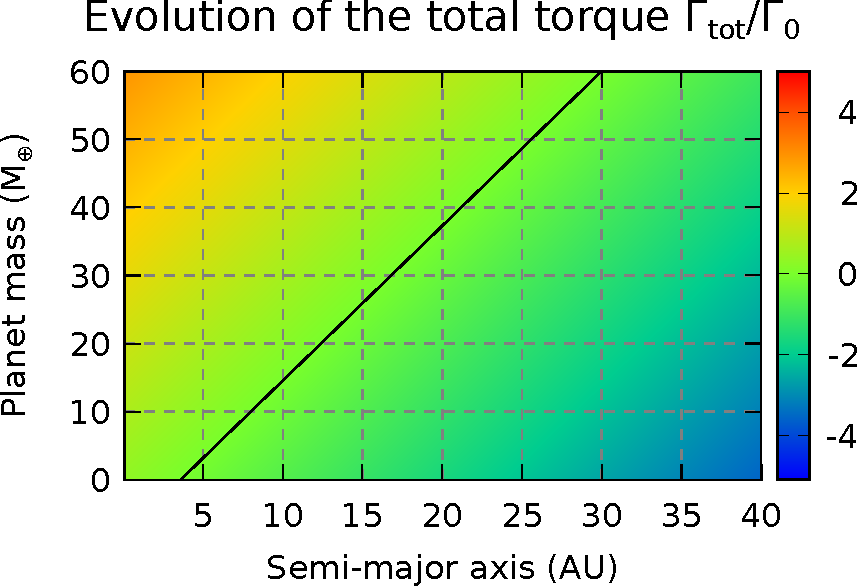
\includegraphics[width=0.65\linewidth]{figure/migration_map/mass_dependant.pdf}
\caption[Carte de migration correspondant à une zone de convergence \textbf{mass\_dependant}.]{Cette carte représente
l'effet du disque dans le cas de l'option \textbf{mass\_dependant} pour une planète en fonction de sa position en abscisse et de
sa masse en ordonnée. La ligne noire représente la zone de couple nul, c'est-à-dire une zone où la migration de la planète
s'arrête.}
\end{figure}

On définit une zone de convergence artificielle qui va dépendre de la masse des planètes. On va donc devoir définir deux bornes en masse et deux bornes en distance orbitale qui vont déterminer cette ligne de couple nul. À l'intérieur (resp. extérieur) de cette séparation virtuelle, la migration sera vers l'extérieur (resp. intérieur).

Ensuite, on définit une pente linéaire plus ou moins importante pour voir à quelle vitesse on va tendre vers la valeur de
saturation à mesure qu'on s'éloigne de la zone de convergence. Une pente de $1$ signifie que le couple $\Gamma/\Gamma_0$
augmente de 1 tous les $10\unit{UA}$.

En résumé, on a ces paramètres suivants à définir : 
\begin{verbatim}
torque_type = mass_dependant

mass_dep_cz_m_max = 30 ! AU
mass_dep_m_max = 60 ! m_earth

mass_dep_cz_m_min = 4 ! AU
mass_dep_m_min = 1 ! m_earth

torque_profile_steepness = 1.0
\end{verbatim}

\subsection{linear\_indep}\label{sec:linear_indep}
Même chose que précédemment, on peut définir un couple artificiel qui définit une zone de convergence indépendante de la masse, c'est-à-dire qu'on ne spécifie que la position de la zone de convergence dans le disque. On a donc : 
\begin{verbatim}
torque_type = linear_indep
indep_cz = 3.0 ! AU
torque_profile_steepness = 1.0
\end{verbatim}

Une pente de $1$ signifie que le couple $\Gamma/\Gamma_0$ augmente de 1 tous les $10\unit{UA}$.

\begin{figure}[htbp]
\centering
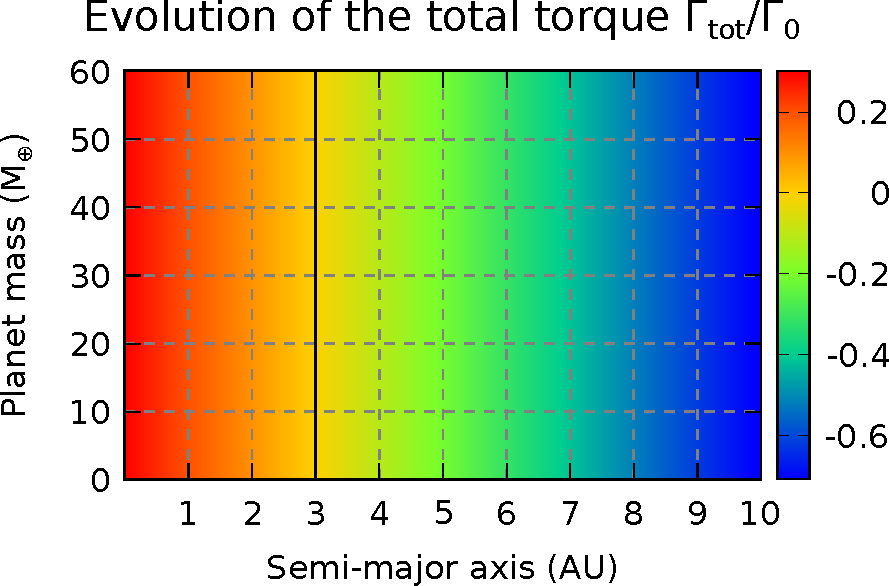
\includegraphics[width=0.65\linewidth]{figure/migration_map/linear_indep.pdf}
\caption[Carte de migration correspondant à une zone de convergence \textbf{linear\_indep}.]{Cette carte représente l'effet du
disque dans le cas de l'option \textbf{linear\_indep} pour une planète en fonction de sa position en abscisse et de sa masse en
ordonnée. La ligne noire représente la zone de couple nul, c'est-à-dire une zone où la migration de la planète s'arrête.}
\end{figure}

\subsection{tanh\_indep}\label{sec:tanh_indep}
Ici, on définit aussi une zone de convergence indépendante de la masse, mais au lieu d'avoir une évolution linéaire du couple à mesure qu'on s'éloigne de la zone de convergence, on a une tangente hyperbolique qui sature à une valeur que l'on peut donner en paramètre. 

La valeur du couple de saturation définit la valeur absolue du couple vers laquelle on va tendre quand on est très loin de la zone de convergence. Si on est à l'extérieur, ce sera cette valeur de saturation prise négativement, tandis que c'est la valeur positive qui est utilisée à l'intérieur.

On a donc les paramètres suivants à définir : 
\begin{verbatim}
torque_type = tanh_indep
indep_cz = 3.0 ! AU
saturation_torque = 1.0 ! in Gamma_0
\end{verbatim}

\begin{figure}[htbp]
\centering
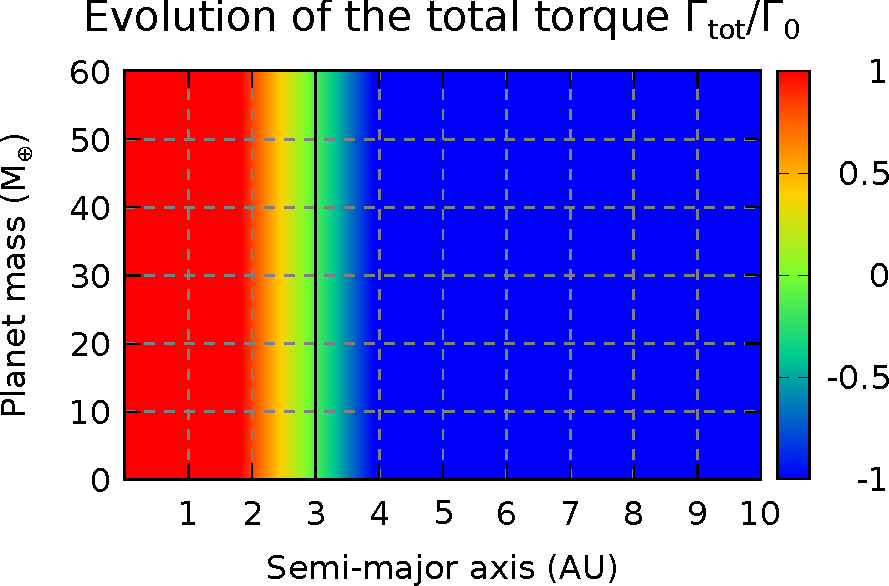
\includegraphics[width=0.65\linewidth]{figure/migration_map/tanh_indep.pdf}
\caption[Carte de migration correspondant à une zone de convergence \textbf{tanh\_indep}.]{Cette carte représente l'effet du
disque dans le cas de l'option \textbf{tanh\_indep} pour une planète en fonction de sa position en abscisse et de sa masse en
ordonnée. La ligne noire représente la zone de couple nul, c'est-à-dire une zone où la migration de la planète s'arrête.}
\end{figure}

\subsection{manual}
Il est aussi possible de rentrer manuellement un couple total en fonction de la position de la planète dans le disque. 

Les valeurs seront alors lues à partir du fichier \textbf{torque\_profile.dat}. La première colonne sera les positions dans le
disque en \unit{UA} tandis que la deuxième colonne sera le couple exercé par le disque en unité de $\Gamma_0$, c'est-à-dire que
l'effet de la masse de la planète sur la vitesse de migration sera toujours pris en compte dans le code au travers de la
dépendance de $\Gamma_0$ en fonction de la masse de la planète et de la masse du disque.

\section{Behind the scene}\label{sec:unitary_tests}
Un programme externe, nommé \textbf{test\_disk.f90} permet d'effectuer des tests unitaires sur différentes fonctions, afin de vérifier quand bon nous semble que chaque fonction n'est pas perturbée par les autres et donne des résultats corrects à la fois physiquement et numériquement.

Les tests génèrent des fichiers de données, et des scripts \textbf{Gnuplot} associés, qu'il suffit ensuite d'exécuter pour avoir le graphique correspondant. 

Les tests que l'on souhaite effectuer sont sélectionnables dans la routine \textbf{unitary\_tests}, où il suffit d'appeler la routine correspondant à un test donné. Sauf quelques cas particuliers, les fichiers de données, scripts Gnuplot et graphiques correspondants sont tous stockés dans le sous-dossier \textbf{unitary\_tests} du dossier d'exécution du binaire de tests.

\subsection{Tests de fonctions}
\subsubsection{test\_alpha\_dz}
Teste la fonction de calcul du paramètre alpha de la viscosité en fonction de la distance, quand une zone morte est modélisée à l'aide de l'option \verb|viscosity = alpha_dz|. Permet de vérifier, via le script \textbf{alpha\_dz.gnuplot}, que le profil de alpha est correct.


\begin{figure}[htbp]
\centering
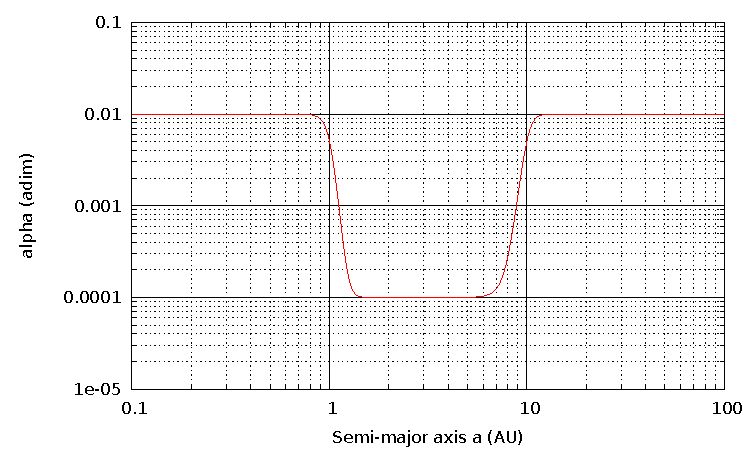
\includegraphics[width=0.65\linewidth]{figure/unitary_tests/alpha_dz.pdf}
\caption{Résultat du test unitaire \textbf{test\_alpha\_dz}.}
\end{figure}

\subsubsection{test\_density\_interpolation}
Teste l'interpolation de la densité de surface entre les valeurs tabulées stockées. Permet aussi de voir la précision du profil en fonction du nombre de points \textbf{nb\_sample} via le script \textbf{density\_interpolation.gnuplot}.

\begin{figure}[htbp]
\centering
\subfloat[Densité de surface]{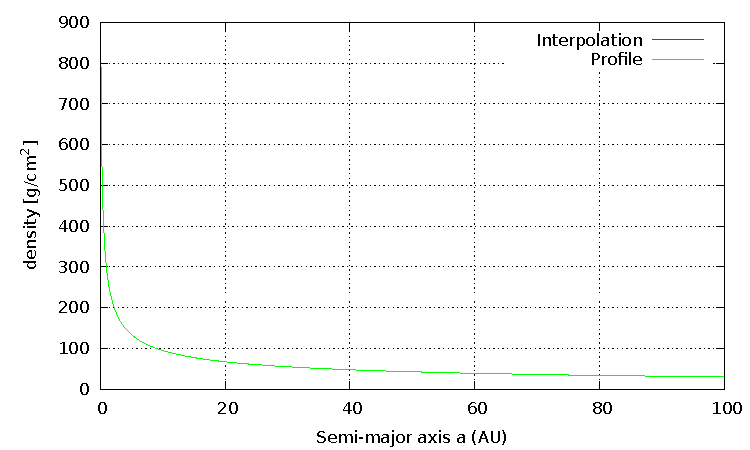
\includegraphics[width=0.49\textwidth]{figure/unitary_tests/density_interpolation.pdf}}\hfill
\subfloat[Indice du profil]{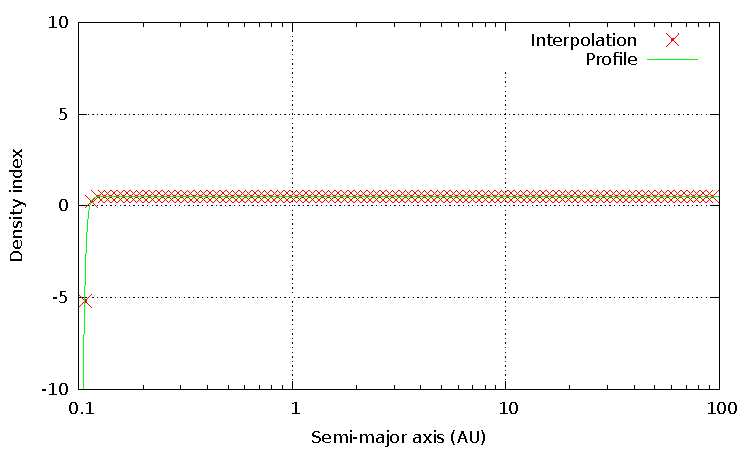
\includegraphics[width=0.49\textwidth]{figure/unitary_tests/density_idx_interpolation.pdf}}

\caption{Résultat du test unitaire \textbf{test\_density\_interpolation}.}
\end{figure}

\subsubsection{test\_function\_zero\_temperature}
Teste la routine qui permet de trouver la température d'équilibre du disque à un point donné, à partir de l'équation de l'énergie. Permet de voir la bistabilité du disque (le fait que plusieurs températures puissent donner lieu à un équilibre, ou le fait qu'aucune température ne donne d'équilibre dans la gamme de température donnée. Le script Gnuplot \textbf{function\_zero\_temperature.gnuplot} affiche le graphique.

\begin{figure}[htbp]
\centering
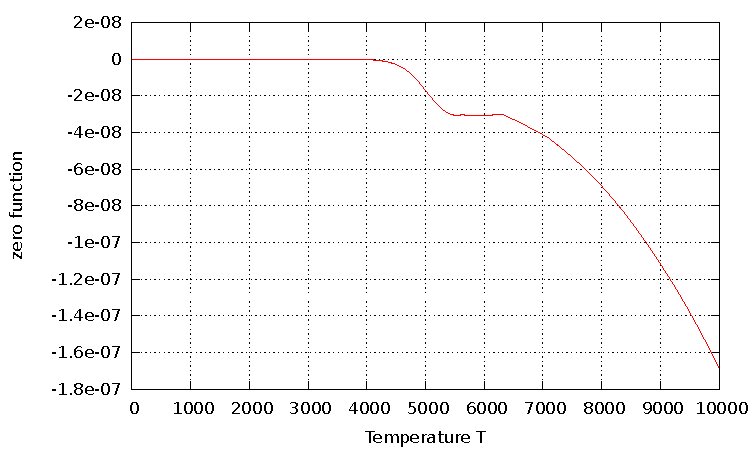
\includegraphics[width=0.65\linewidth]{figure/unitary_tests/function_zero_temperature.pdf}
\caption{Résultat du test unitaire \textbf{test\_function\_zero\_temperature}.}
\end{figure}

\subsubsection{test\_functions\_FGK}
Affiche les fonctions $F$, $G$, et $K$ définies dans \cite{paardekooper2011torque} via le script \textbf{functions\_FGK.gnuplot}.

\begin{figure}[htbp]
\centering
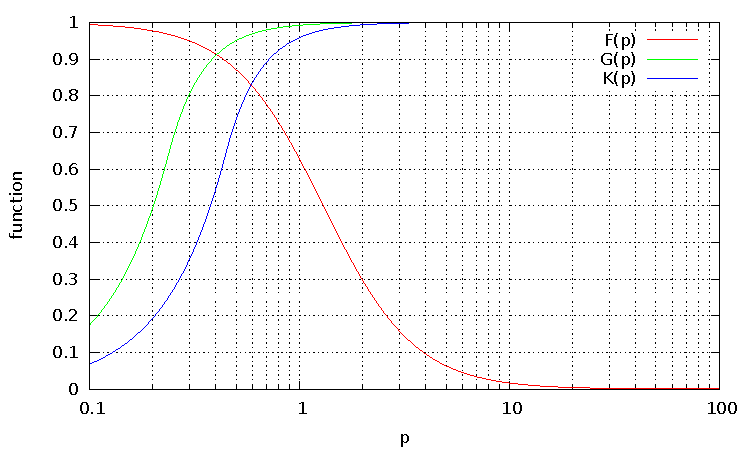
\includegraphics[width=0.65\linewidth]{figure/unitary_tests/functions_FGK.pdf}
\caption{Résultat du test unitaire \textbf{test\_functions\_FGK}.}
\end{figure}

\subsubsection{test\_manual\_torque\_interpolation}
Dans le cas où le profil de couple en fonction de la distance est manuel, teste l'interpolation du couple entre les points de la discrétisation de ce dernier. Le script Gnuplot \textbf{torque\_interpolation.gnuplot} permet d'afficher les résultats du test.

\begin{figure}[htbp]
\centering
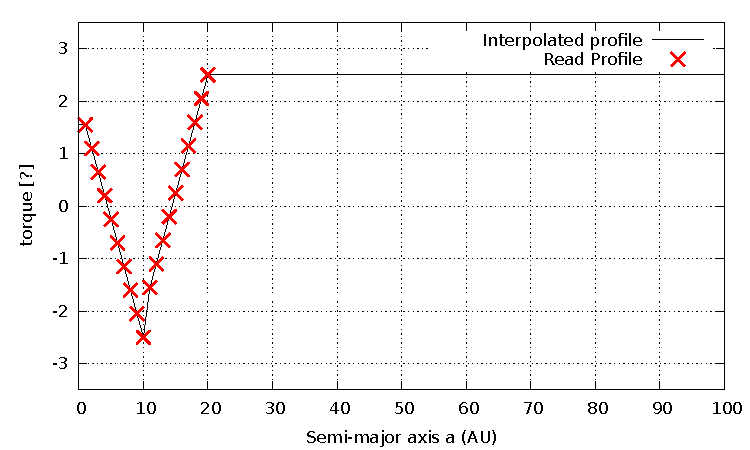
\includegraphics[width=0.65\linewidth]{figure/unitary_tests/torque_interpolation.pdf}
\caption{Résultat du test unitaire \textbf{test\_manual\_torque\_interpolation}.}
\end{figure}

\subsubsection{test\_retrieval\_of\_orbital\_elements}
Teste si pour des orbites circulaires de demi-grands axes différents, les éléments orbitaux sont bien retrouvés. Les scripts Gnuplot pour $a$, $e$, et $I$ sont respectivement \textbf{retrieval\_a.gnuplot}, \textbf{retrieval\_e.gnuplot} et \textbf{retrieval\_I.gnuplot}.

\begin{figure}[htbp]
\centering
\subfloat[Demi-grand axe $a$]{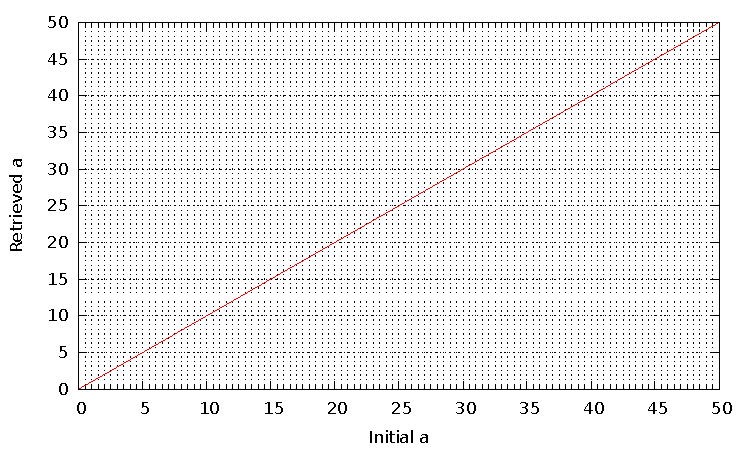
\includegraphics[width=0.49\textwidth]{figure/unitary_tests/retrieval_a.pdf}}\hfill
\subfloat[Excentricité $e$]{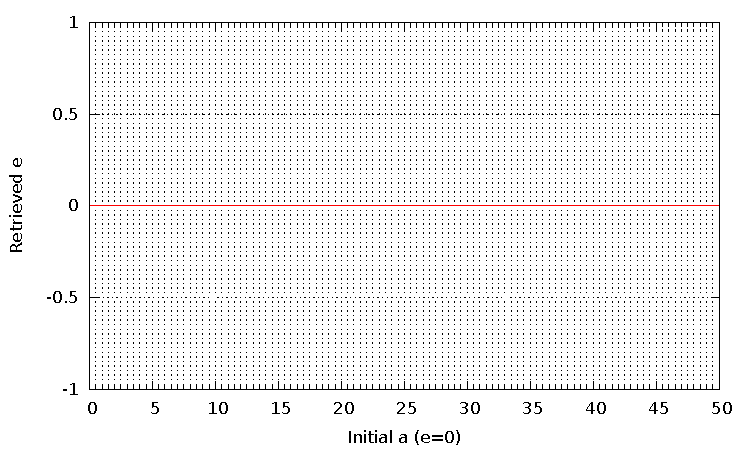
\includegraphics[width=0.49\textwidth]{figure/unitary_tests/retrieval_e.pdf}}

\subfloat[Inclinaison $I$]{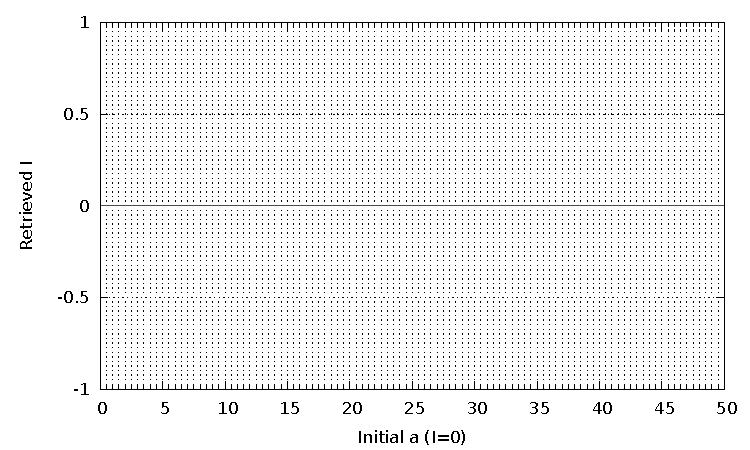
\includegraphics[width=0.49\textwidth]{figure/unitary_tests/retrieval_I.pdf}}
\caption{Résultat du test unitaire \textbf{test\_retrieval\_of\_orbital\_elements}.}
\end{figure}

\subsubsection{test\_temperature\_interpolation}
Teste l'interpolation de la température entre les points de la discrétisation radiale du profil. Le script Gnuplot correspondant est \textbf{temperature\_interpolation.gnuplot}.

\begin{figure}[htbp]
\centering
\subfloat[Température]{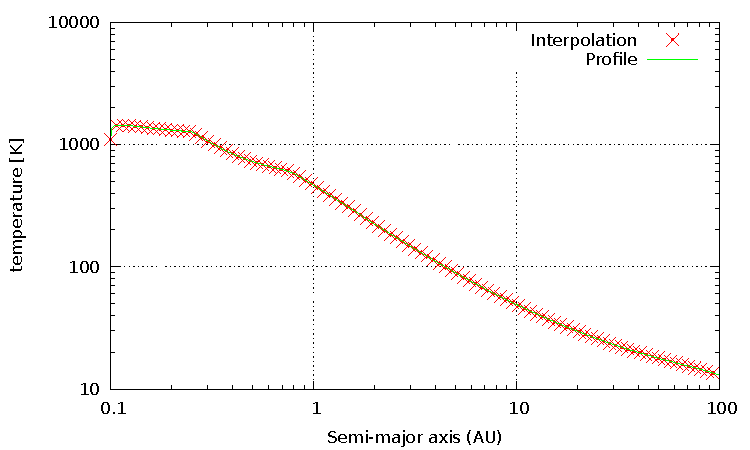
\includegraphics[width=0.49\textwidth]{figure/unitary_tests/temperature_interpolation.pdf}}\hfill
\subfloat[Indice du profil]{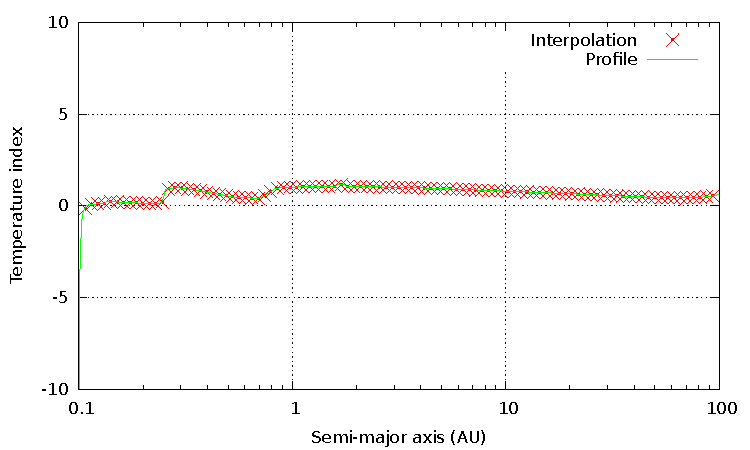
\includegraphics[width=0.49\textwidth]{figure/unitary_tests/temperature_idx_interpolation.pdf}}
\caption{Résultat du test
unitaire \textbf{test\_temperature\_interpolation}.}
\end{figure}

\begin{figure}[htbp]
\centering
\subfloat[Diffusivité
thermique]{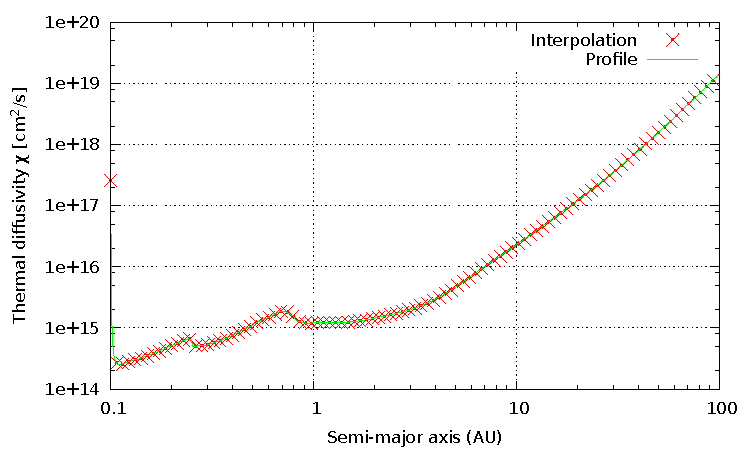
\includegraphics[width=0.49\textwidth]{figure/unitary_tests/diffusivity_interpolation.pdf}}\hfill
\subfloat[Échelle de hauteur]{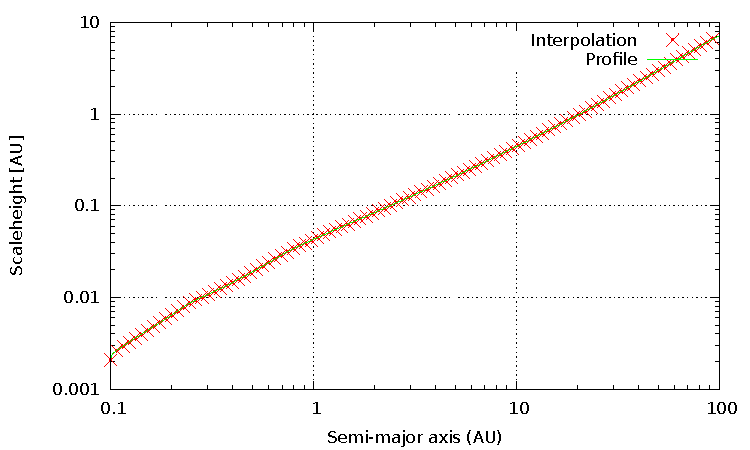
\includegraphics[width=0.49\textwidth]{figure/unitary_tests/scaleheight_interpolation.pdf}}

\subfloat[Viscosité]{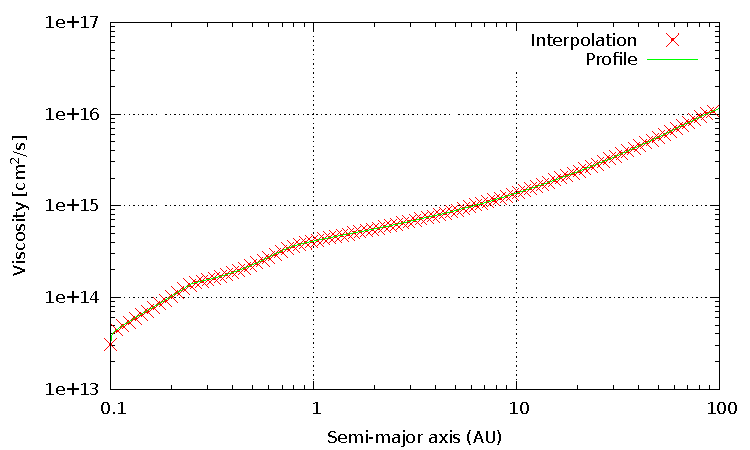
\includegraphics[width=0.49\textwidth]{figure/unitary_tests/viscosity_interpolation.pdf}}
\caption{Autres profils du test unitaire \textbf{test\_temperature\_interpolation}.}
\end{figure}

\subsection{Test de paramètres physiques}
Les tests ont été effectués pour les valeurs du disque de référence \refsec{sec:reference_disk}.

\subsubsection{study\_ecc\_corot}
Pour une planète de masse et position fixées, évolution du préfacteur d'atténuation du couple de corotation $E$, où
$\Gamma_\text{tot}=\Gamma_0 (\Gamma_L + E * \Gamma_c)$. Le fichier Gnuplot correspondant est \textbf{ecc\_corot.gnuplot}. 

\begin{figure}[htbp]
\centering
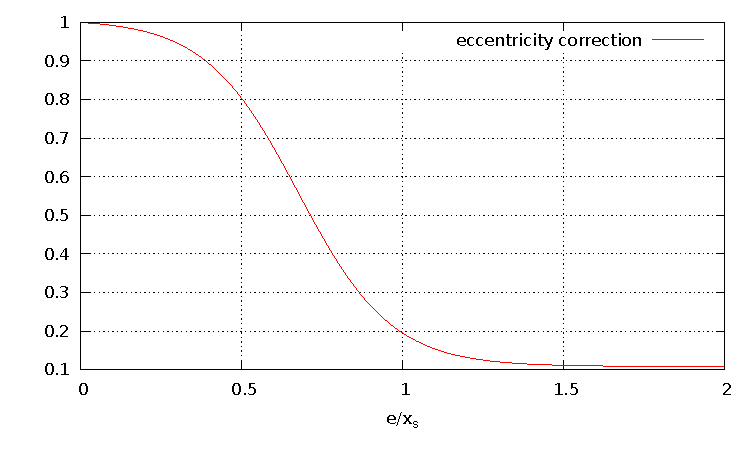
\includegraphics[width=0.65\linewidth]{figure/unitary_tests/ecc_corot.pdf}
\caption{Résultat du test unitaire \textbf{study\_ecc\_corot}.}
\end{figure}

\subsubsection{study\_eccentricity\_effect\_on\_corotation}
Pour une planète de masse et position fixées, évolution du couple de corotation en fonction de l'excentricité. Le fichier
Gnuplot correspondant est \textbf{eccentricity\_effect\_on\_corotation.gnuplot}. 

\begin{figure}[htbp]
\centering
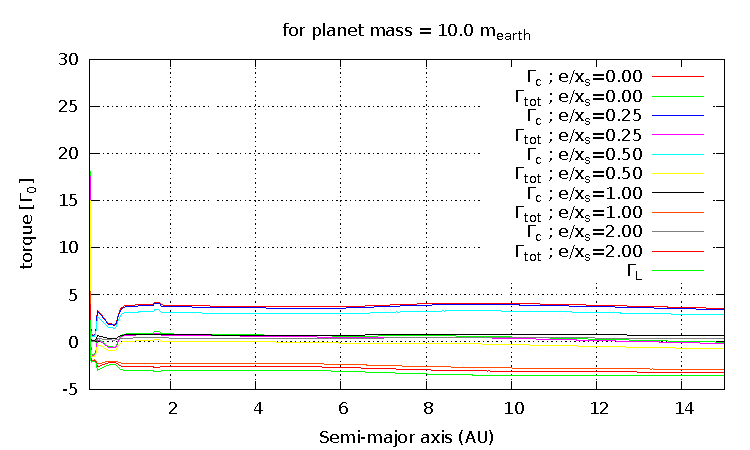
\includegraphics[width=0.65\linewidth]{figure/unitary_tests/eccentricity_effect_on_corotation.pdf}
\caption{Résultat du test unitaire \textbf{study\_eccentricity\_effect\_on\_corotation}.}
\end{figure}

\subsubsection{study\_opacity\_profile}
Affiche pour différentes densités volumiques, le profil d'opacité $\kappa$ en fonction de la température.  Le fichier Gnuplot
correspondant est \textbf{opacity.gnuplot}. Le fichier \textbf{opacity\_comparison.gnuplot} compare quant à lui les opacités de
\cite{bell1994FU} et \cite{zhu2009nonsteady}. 

\begin{figure}[htbp]
\centering
\subfloat[Opacité de \cite{hure2000transition}]{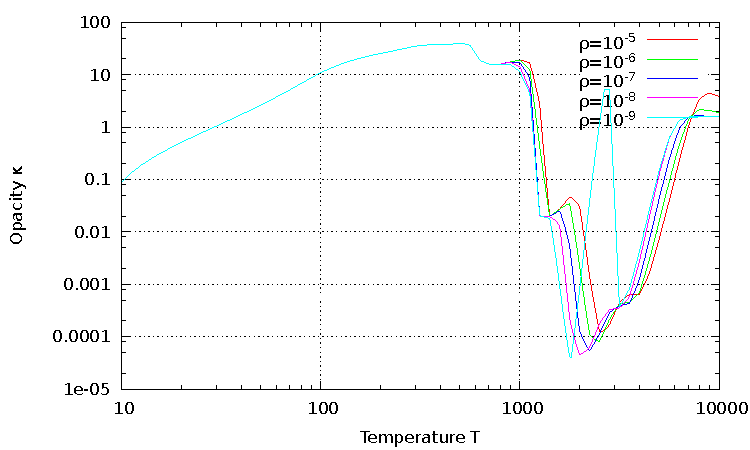
\includegraphics[width=0.49\textwidth]{figure/unitary_tests/opacity.pdf}}\hfill
\subfloat[Opacités de \cite{bell1994FU} et \cite{zhu2009nonsteady}]{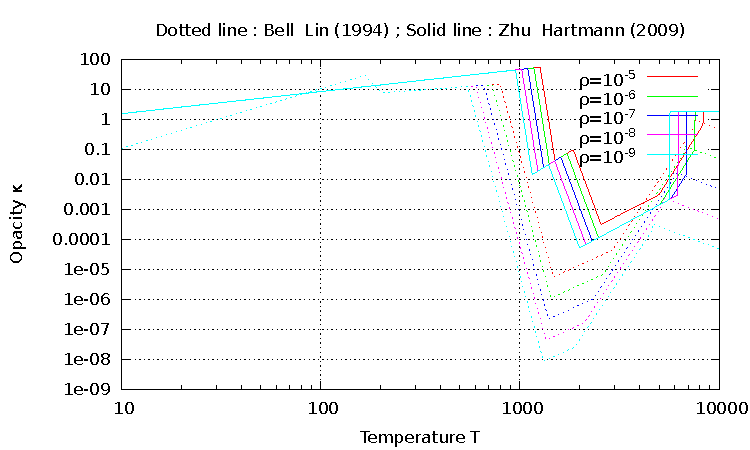
\includegraphics[width=0.49\textwidth]{figure/unitary_tests/opacity_comparison.pdf}}

\caption{Résultat du test unitaire \textbf{study\_opacity\_profile}.}
\end{figure}

\subsubsection{study\_optical\_depth\_profile}
Affiche le profil de profondeur optique $\tau$ du disque. Le fichier Gnuplot correspondant est \textbf{optical\_depth\_profile.gnuplot}. 

\begin{figure}[htbp]
\centering
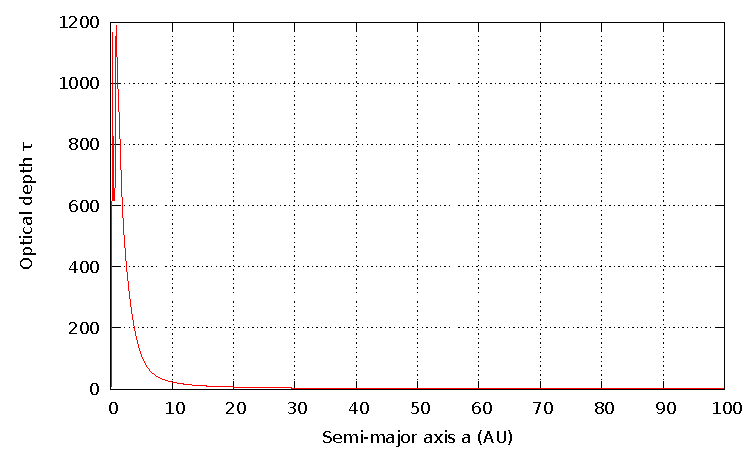
\includegraphics[width=0.65\linewidth]{figure/unitary_tests/optical_depth_profile.pdf}
\caption{Résultat du test unitaire \textbf{study\_optical\_depth\_profile}.}
\end{figure}

\subsubsection{study\_scaleheight\_profile}
Affiche le profil d'échelle de hauteur $H$et de rapport d'aspect $h$ du disque, respectivement via les fichiers Gnuplot \textbf{scaleheight\_profile.gnuplot} et \textbf{aspect\_ratio.gnuplot}.

\begin{figure}[htbp]
\centering
\subfloat[Échelle de hauteur $H$]{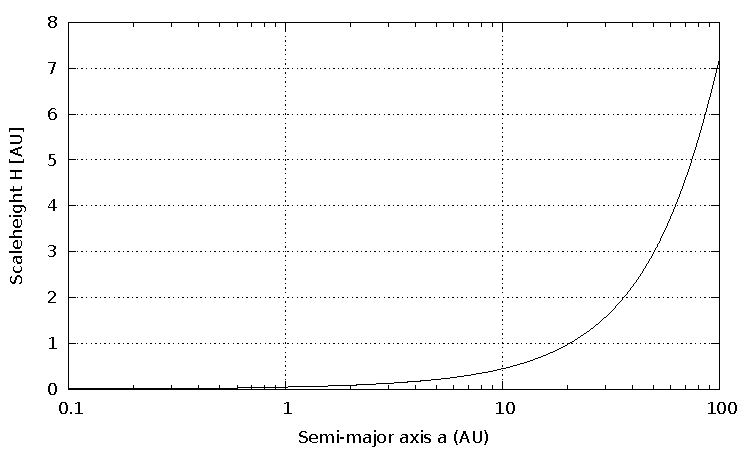
\includegraphics[width=0.49\textwidth]{figure/unitary_tests/scaleheight_profile.pdf}}\hfill
\subfloat[Rapport d'aspect $h$]{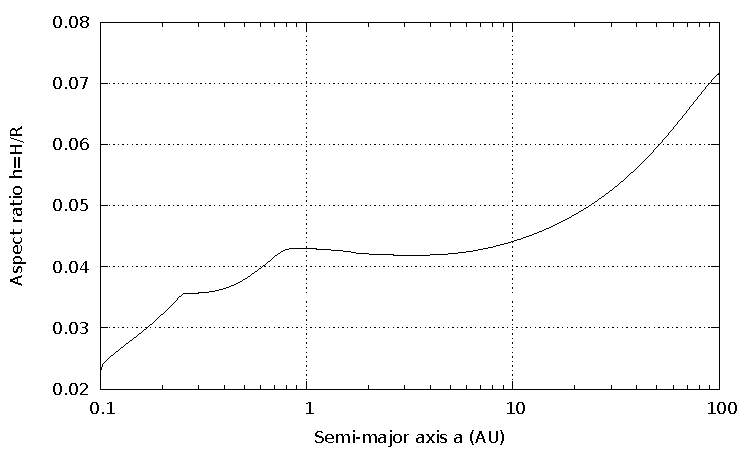
\includegraphics[width=0.49\textwidth]{figure/unitary_tests/aspect_ratio_profile.pdf}}\hfill
\caption{Résultat du test unitaire \textbf{study\_scaleheight\_profile}.}
\end{figure}

\subsubsection{study\_temperature\_profile}
Affiche le profil de température du disque via les fichiers Gnuplot \textbf{temperature\_profile.gnuplot} et \textbf{temperature\_index.gnuplot}.

\begin{figure}[htbp]
\centering
\subfloat[Profil de température]{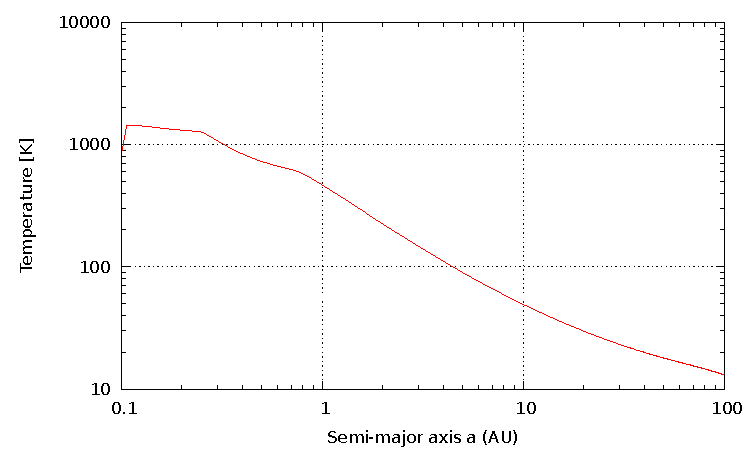
\includegraphics[width=0.49\textwidth]{figure/unitary_tests/temperature_profile.pdf}}\hfill
\subfloat[Indice négatif du profil de température]{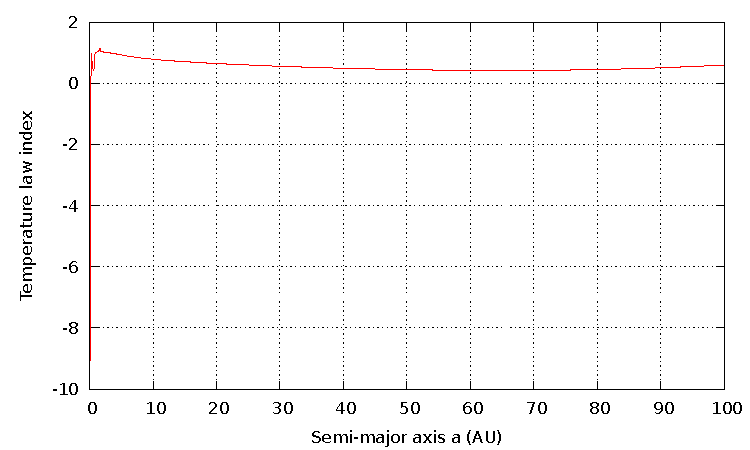
\includegraphics[width=0.49\textwidth]{figure/unitary_tests/temperature_index.pdf}}
\caption{Résultat du test unitaire \textbf{study\_temperature\_profile}.}
\end{figure}

\subsubsection{study\_thermal\_diffusivity\_profile}
Affiche le profil de diffusivité thermique $\chi$ du disque via le fichier Gnuplot \textbf{thermal\_diffusivity\_profile.gnuplot}.

\begin{figure}[htbp]
\centering
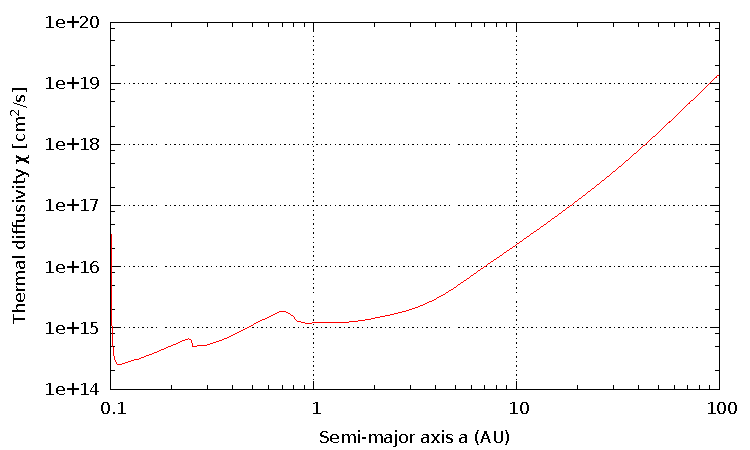
\includegraphics[width=0.65\linewidth]{figure/unitary_tests/thermal_diffusivity_profile.pdf}
\caption{Résultat du test unitaire \textbf{study\_thermal\_diffusivity\_profile}.}
\end{figure}

\subsubsection{study\_torques}
Affiche la carte de migration du disque via les fichiers gnuplot \textbf{corotation\_torque.gnuplot}, \textbf{total\_torque.gnuplot}, \textbf{total\_torque\_units.gnuplot}, \textbf{lindblad\_torque.gnuplot} et \textbf{ref\_torque.gnuplot} qui affichent respectivement $\Gamma_c$, $Gamma_\text{tot}/\Gamma_0$, $\Gamma_\text{tot}$, $\Gamma_L$ et $\Gamma_0$.

Les cartes de migration sont présentées \refsec{sec:chap3}.

\subsubsection{study\_torques\_fixed\_a}
Affichage du couple pour une planète de masse variable, mais dont la position est fixe. \textbf{torques\_fixed\_a.gnuplot}, \textbf{ref\_torque\_fixed\_a.gnuplot}, \textbf{torques\_fixed\_a\_units.gnuplot} et \textbf{specific\_torque\_fixed\_a.gnuplot} affichent respectivement $Gamma_\text{tot}/\Gamma_0$, $\Gamma_0$, $\Gamma_\text{tot}$ et le couple total spécifique, en unité de Jupiter (distance notamment). 

\begin{figure}[htbp]
\centering
\subfloat[$Gamma_\text{tot}/\Gamma_0$]{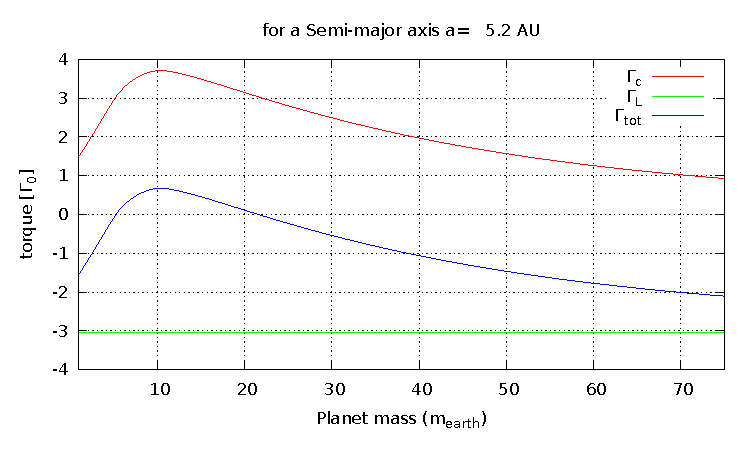
\includegraphics[width=0.49\textwidth]{figure/unitary_tests/torques_fixed_a.pdf}}\hfill
\subfloat[$\Gamma_\text{tot}$]{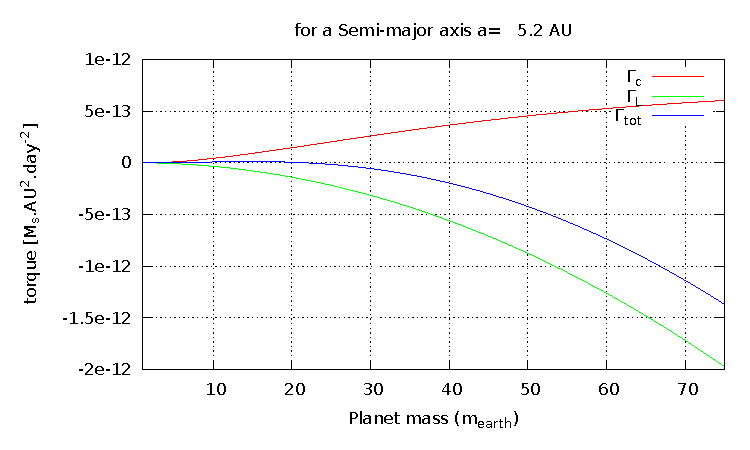
\includegraphics[width=0.49\textwidth]{figure/unitary_tests/torques_fixed_a_units.pdf}}

\subfloat[$\Gamma_0$]{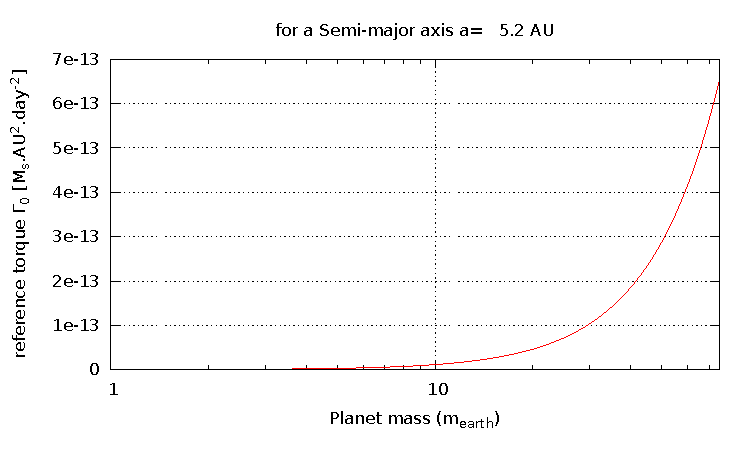
\includegraphics[width=0.49\textwidth]{figure/unitary_tests/ref_torque_fixed_a.pdf}}\hfill
\subfloat[Couple spécifique]{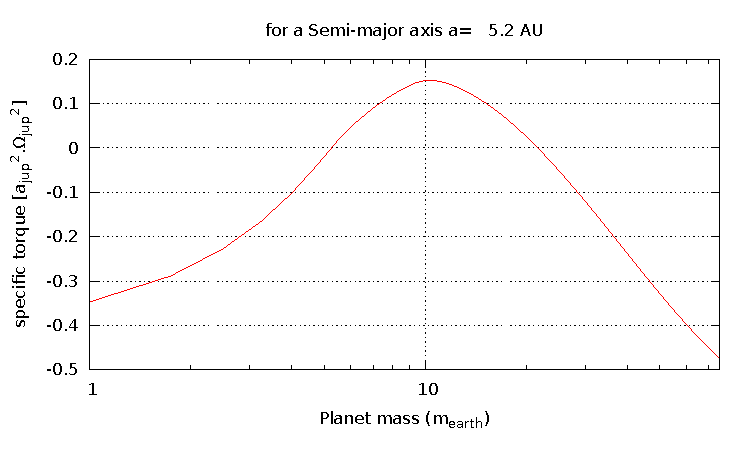
\includegraphics[width=0.49\textwidth]{figure/unitary_tests/specific_torque_fixed_a.pdf}}
\caption{Résultat du test unitaire \textbf{study\_torques\_fixed\_a}.}
\end{figure}

\subsubsection{study\_torques\_fixed\_m}
Le couple total ressenti par une planète de masse donnée est affiché via les scripts Gnuplot \textbf{torques\_fixed\_m.gnuplot}, \textbf{ref\_torque\_fixed\_m.gnuplot} et \textbf{torques\_fixed\_m\_units.gnuplot} qui affichent respectivement $Gamma_\text{tot}/\Gamma_0$, $\Gamma_0$ et $\Gamma_\text{tot}$.

\begin{figure}[htbp]
\centering
\subfloat[$Gamma_\text{tot}/\Gamma_0$]{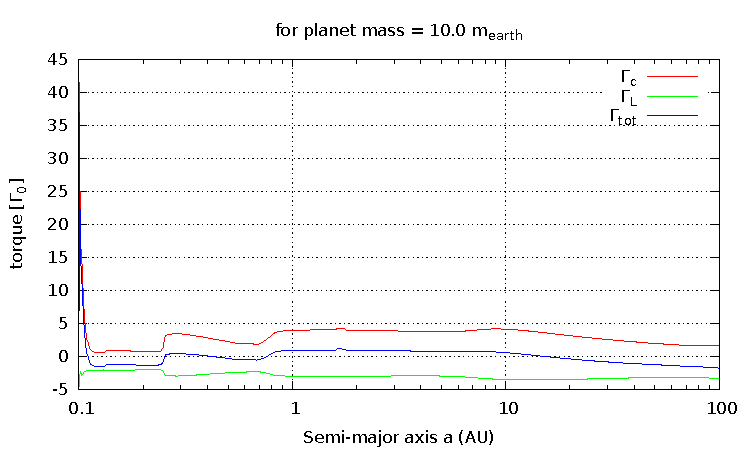
\includegraphics[width=0.49\textwidth]{figure/unitary_tests/torques_fixed_m.pdf}}\hfill
\subfloat[$\Gamma_\text{tot}$]{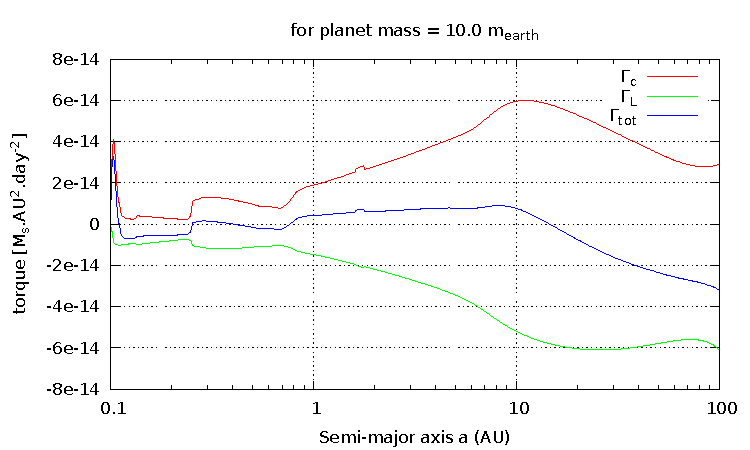
\includegraphics[width=0.49\textwidth]{figure/unitary_tests/torques_fixed_m_units.pdf}}

\subfloat[$\Gamma_0$]{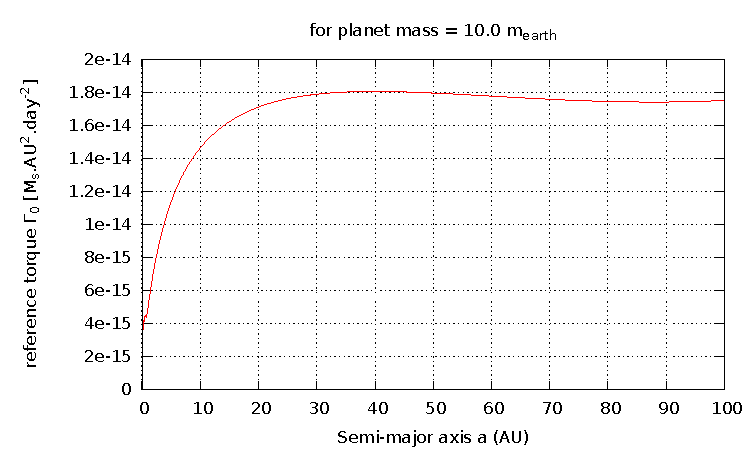
\includegraphics[width=0.49\textwidth]{figure/unitary_tests/ref_torque_fixed_m.pdf}}
\caption{Résultat du test unitaire \textbf{study\_torques\_fixed\_m}.}
\end{figure}

\subsubsection{study\_viscosity}
Affiche le profil de viscosité du disque via \textbf{viscosity.gnuplot}.

\begin{figure}[htbp]
\centering
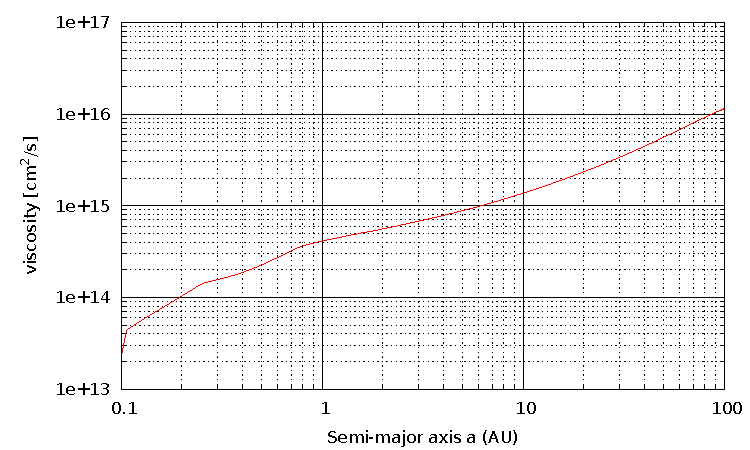
\includegraphics[width=0.65\linewidth]{figure/unitary_tests/viscosity.pdf}
\caption{Résultat du test unitaire \textbf{study\_viscosity}.}
\end{figure}

\subsubsection{test\_turbulence\_mode}
Génère et stocke les valeurs de $10000$ modes de turbulence, afin d'en vérifier les propriétés statistiques. Les données sont stockées dans le fichier \textbf{turbulence\_mode.dat} où dans l'ordre des colonnes sont stockés le mode $m$, les positions $(r;\phi)$ du mode, le temps de vie du mode, l'extension radiale $\Delta R$ du mode ainsi que le préfacteur adimensionné $\chi$ correspondant \citep[pour plus de détails]{ogihara2007accretion}. 

\subsubsection{test\_turbulence\_torque}
Teste la turbulence. En particulier le script Gnuplot \textbf{turbulence\_torque.gnuplot} affiche l'histogramme du couple turbulent et le compare à l'histogramme attendu. 

\begin{figure}[htbp]
\centering
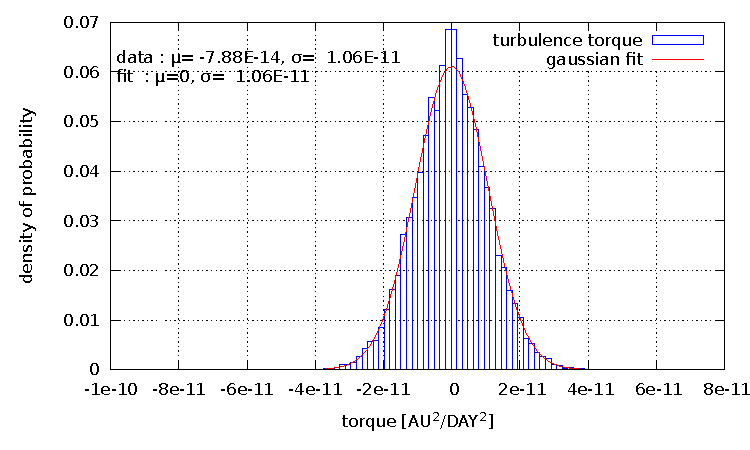
\includegraphics[width=0.65\linewidth]{figure/unitary_tests/turbulence_torque.pdf}
\caption{Résultat du test unitaire \textbf{test\_turbulence\_torque}.}
\end{figure}

\subsubsection{study\_dissipation\_at\_one\_location}
L'évolution de la densité de surface en un point donné du disque quand la dissipation est active (quel que soit le type de dissipation). Le fichier Gnuplot correspondant est \textbf{local\_density\_dissipation.gnuplot}. 

\subsubsection{study\_influence\_of\_dissipation\_on\_torque}
Montre l'évolution de la carte de migration au fur et à mesure de la dissipation du disque. Les cartes sont stockées dans un sous-dossier \textbf{dissipation} du dossier courant. Le fichier Gnuplot correspondant est \textbf{total\_torque.gnuplot} dans le dossier \textbf{dissipation}. 


\subsubsection{test\_disk\_dissipation}
Teste la dissipation du disque dans un sous-dossier \textbf{dissipation} du dossier \textbf{unitary\_tests}. Le script Gnuplot \textbf{density.gnuplot} génère différentes images du profil de densité de surface du disque au cours du temps.


\subsection{Débogage}
Afin de déboguer le code, certaines routines ont été créées spécialement à cet effet. 

Dans le module \textbf{turbulence.f90}, la routine \textbf{print\_turbulencemode\_properties} permet d'afficher les propriétés d'un mode donné, passé en argument. Ce mode est alors une instance de la structure de type \texttt{TurbulenceMode}. 

Dans le module \textbf{user\_module.f90}, la routine \textbf{debug\_infos} permet d'afficher un maximum d'informations pour le
pas de temps courant. À utiliser dans une boucle de test afin de ne l'afficher qu'à certains instants, sous peine de saturer
l'affichage. 

De plus, la routine \textbf{print\_planet\_properties} permet d'afficher les informations d'une planète, définies dans une structure du type \textbf{PlanetProperties}.

Un exemple de code de débogage est donc la suite d'instructions suivante :
\begin{lstlisting}[language=Fortran]
if (time.gt.365.25) then
  if ((p_prop%eccentricity.lt.ECCENTRICITY_CUTOFF).and.(p_prop%radius.gt.INNER_BOUNDARY_RADIUS)) then
  
    call debug_infos(time, n_bodies, planet, position, velocity, acceleration, &
                 time_mig, migration_acceleration, time_ecc, eccentricity_acceleration, &
                 turbulence_acceleration, corotation_torque, lindblad_torque, torque_ref, ecc_corot)
  end if
  open(12, file="debug.out", access='append')
  write (12,*) "time = ", time, " ; planet", planet
  call print_planet_properties(p_prop, output=12)
  close(12)
  stop
end if
\end{lstlisting}
